\section*{Problem 3}
	\begin{proof} [Solution]
		We can guess that if $p_r$ increases, then $\mu(t)$ also increases. Increasing $p_r$ means that each particle can move further to the right. But $\sigma^2$ is different. It is based on the difference between $p_r$ and $p_l$. Because, $p_r$ means `move to the right' and $p_l$ `means move to the left'. We can think of them as a force acting in opposite directions. If there is no difference between the two values, the force will be balanced and particles can spread to various places based on the center. However, if the force on one side is strong, particles are concentrated around that side.\\
		The result below is analyzed numerically by varying $p_r$ from 0 to 1.
		\begin{center}
			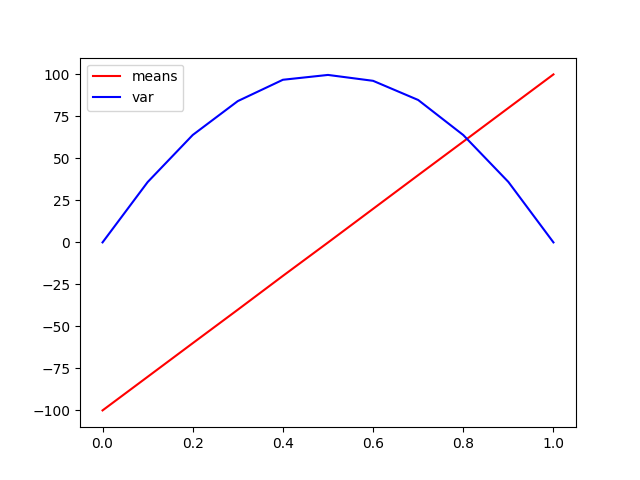
\includegraphics[width=0.7\textwidth]{mean_var.png}
		\end{center}
	\end{proof}